\section{Padrões de Affordance}

\begin{frame}{Padrões de Affordance}
\begin{block}{Toque}
  \begin{itemize}
    \item<1-> É uma técnica de design visual que usa relevos e/ou sombras para fazer com que certos elementos pareçam palpáveis. Mas é necessário que seu uso seja aplicado corretamente e com consistência.
  \end{itemize}
\end{block}
\end{frame}
%%%%%%%%%%%%%%%%

\begin{frame}{Padrões de Affordance}
\begin{block}{Toque}
    \begin{figure}
    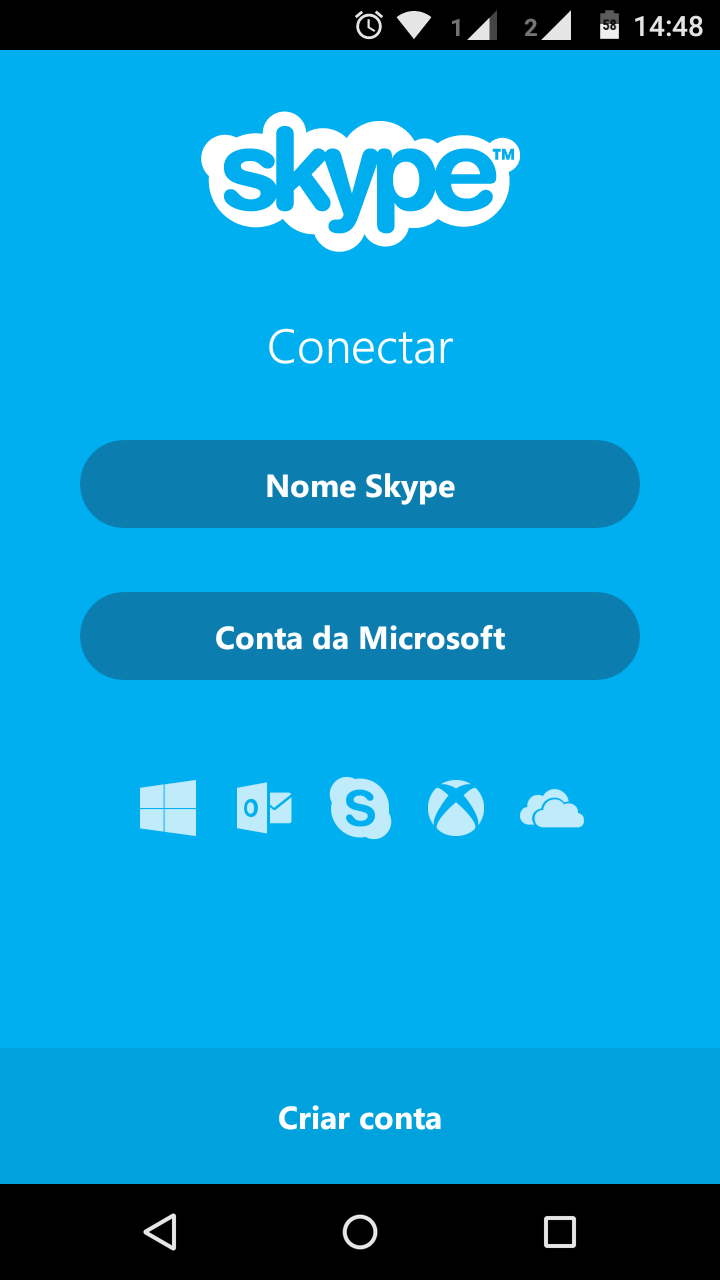
\includegraphics[width=3cm]{figuras/touch/tocar}
    \end{figure}
\end{block}
\end{frame}
%%%%%%%%%%%%%%%%

\begin{frame}{Padrões de Affordance}
\begin{block}{Toque}
    \begin{figure}
    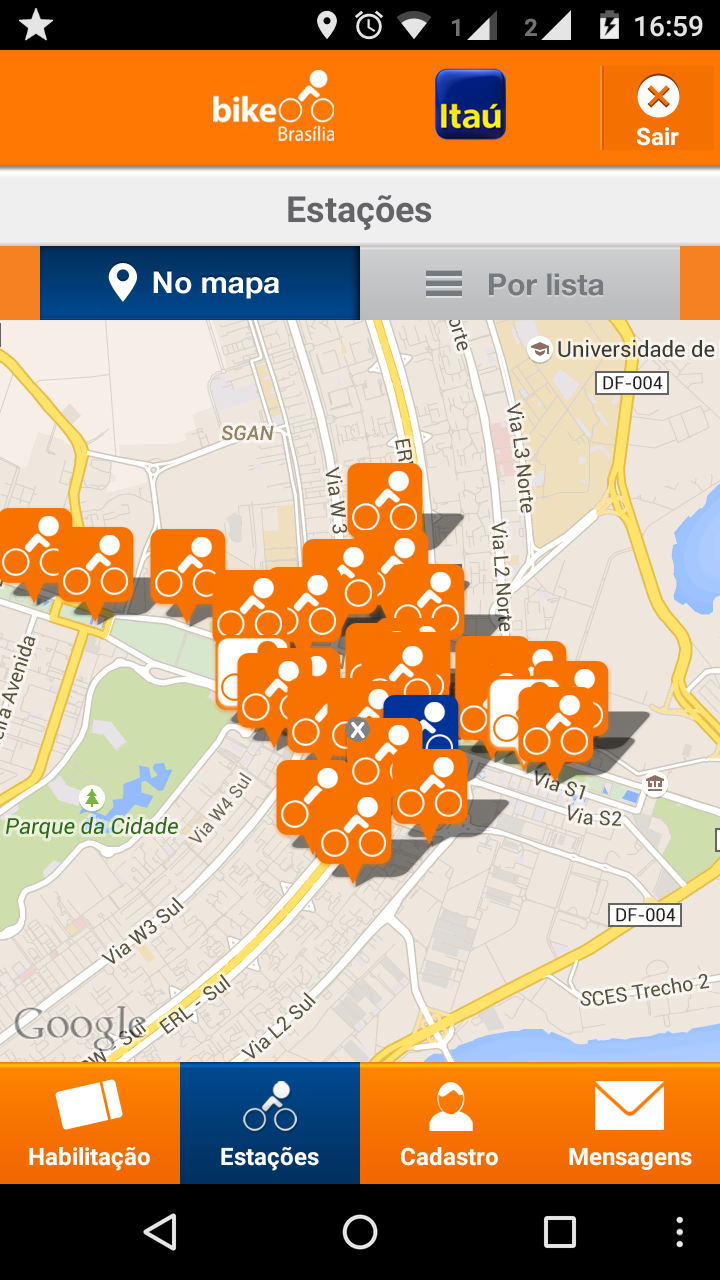
\includegraphics[width=3cm]{figuras/touch/tocar3}
    \end{figure}
\end{block}
\end{frame}
%%%%%%%%%%%%%%%%

\begin{frame}{Padrões de Affordance}
\begin{block}{Toque}
    \begin{figure}
    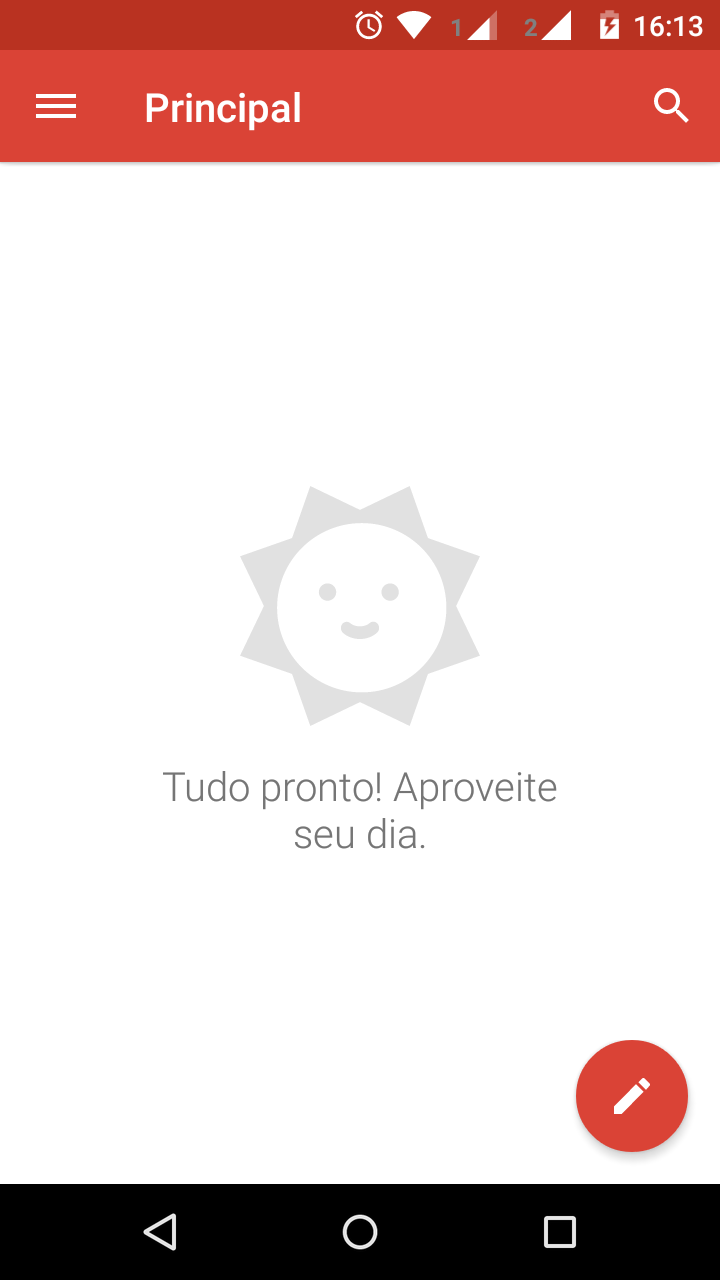
\includegraphics[width=3cm]{figuras/touch/tocar2}
    \end{figure}
\end{block}
\end{frame}
%%%%%%%%%%%%%%%%

\begin{frame}{Padrões de Affordance}
\begin{block}{Deslizar}
  \begin{itemize}
    \item<1-> Essa técnica tem como objetivo indicar ao usuário a possibilidade de que haja mais itens para se ver.
  \end{itemize}
\end{block}
\end{frame}
%%%%%%%%%%%%%%%%

\begin{frame}{Padrões de Affordance}
\begin{block}{Deslizar}
    \begin{figure}
    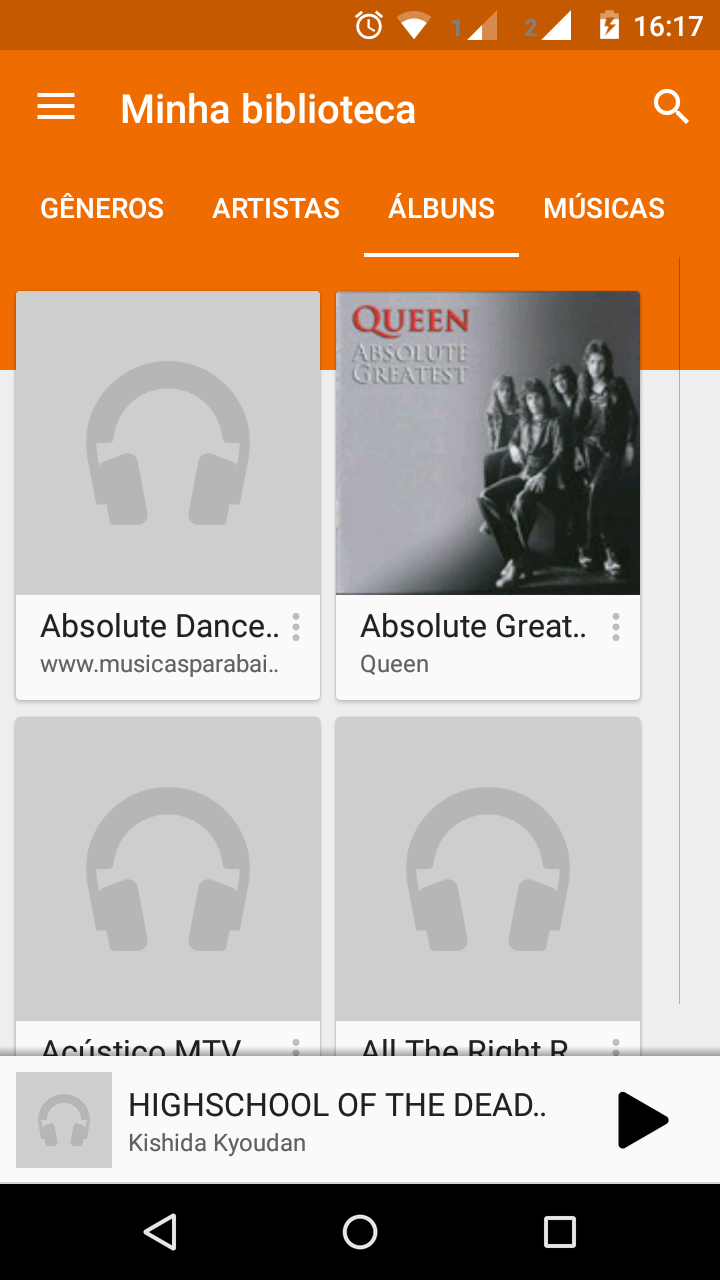
\includegraphics[width=3cm]{figuras/deslize/deslize2}
    \end{figure}
\end{block}
\end{frame}
%%%%%%%%%%%%%%%%

\begin{frame}{Padrões de Affordance}
\begin{block}{Deslizar}
    \begin{figure}
    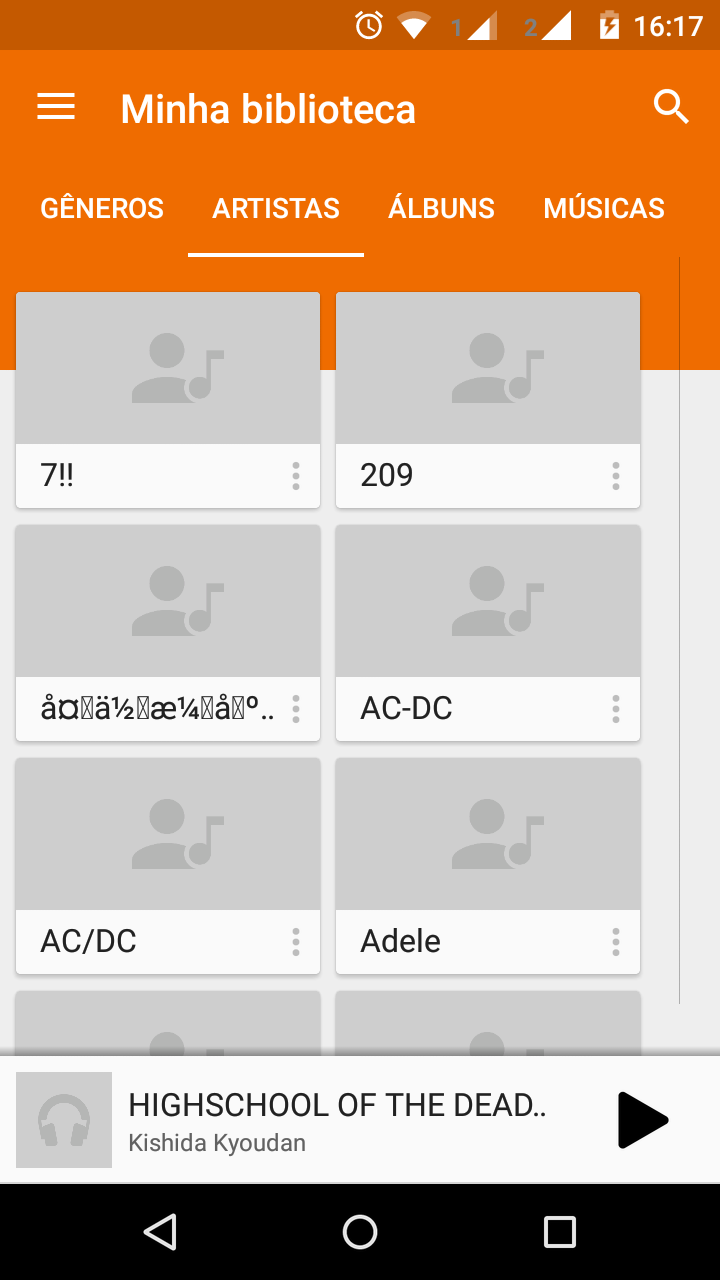
\includegraphics[width=3cm]{figuras/deslize/deslize3}
    \end{figure}
\end{block}
\end{frame}
%%%%%%%%%%%%%%%%

\begin{frame}{Padrões de Affordance}
\begin{block}{Deslizar}
    \begin{figure}
    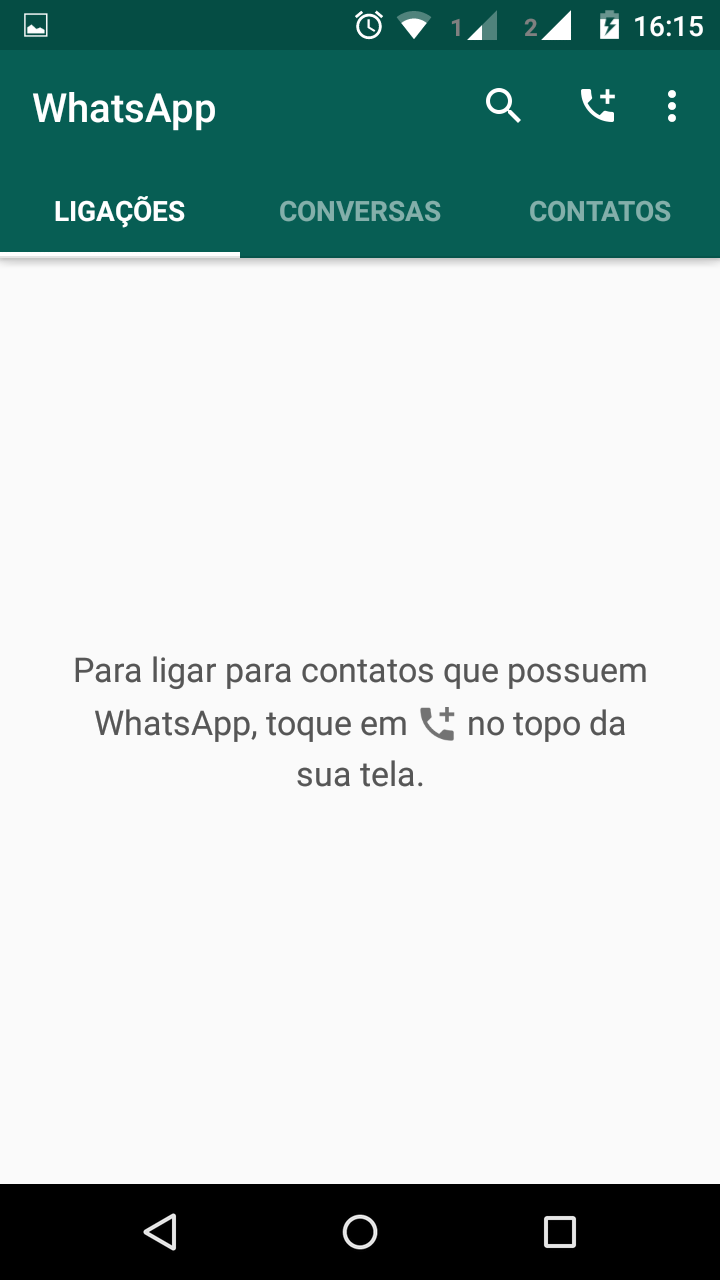
\includegraphics[width=3cm]{figuras/deslize/deslize1}
    \end{figure}
\end{block}
\end{frame}
%%%%%%%%%%%%%%%%

\begin{frame}{Padrões de Affordance}
\begin{block}{Deslizar}
    \begin{figure}
    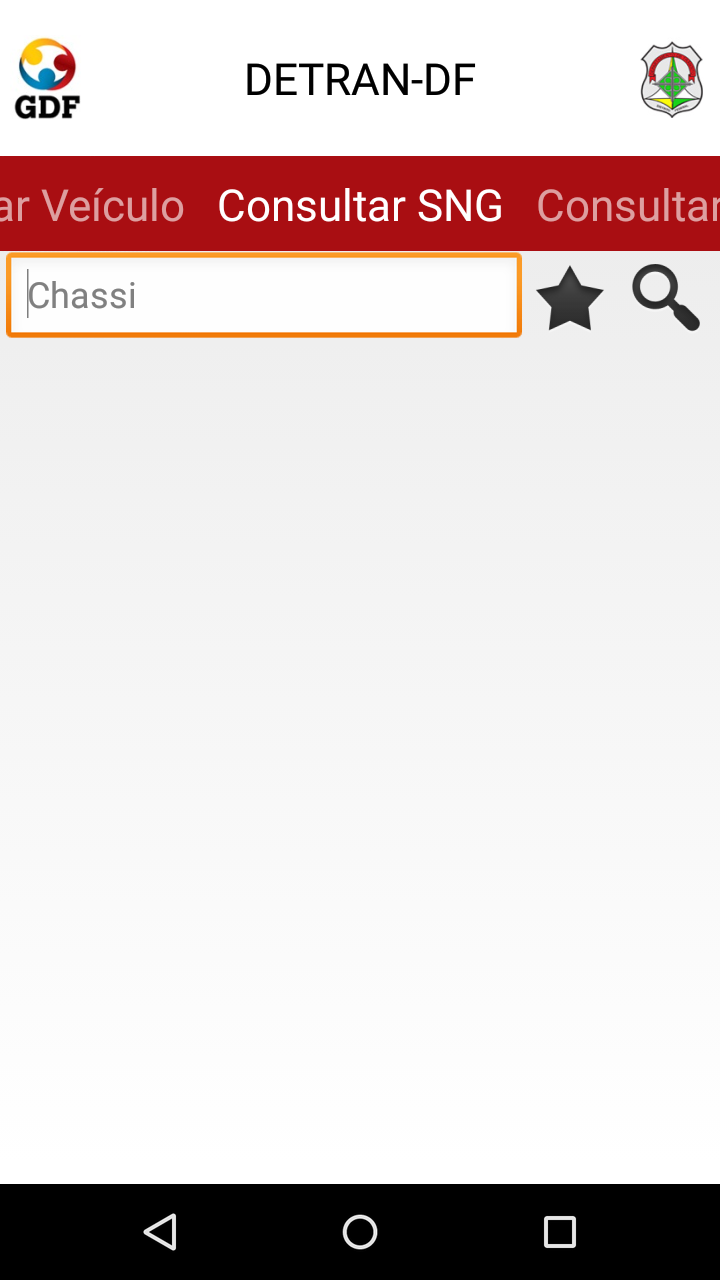
\includegraphics[width=3cm]{figuras/deslize/deslize6}
    \end{figure}
\end{block}
\end{frame}
%%%%%%%%%%%%%%%%

\begin{frame}{Padrões de Affordance}
\begin{block}{Deslizar}
    \begin{figure}
    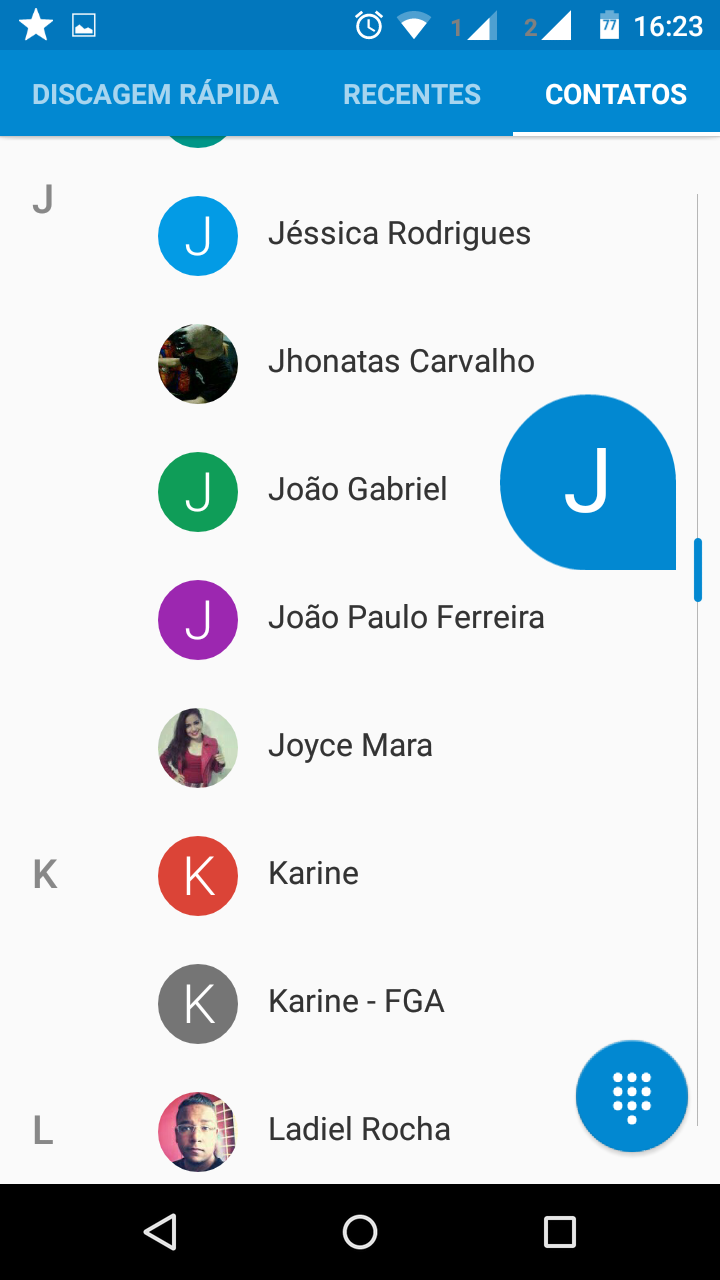
\includegraphics[width=3cm]{figuras/deslize/deslize5}
    \end{figure}
\end{block}
\end{frame}
%%%%%%%%%%%%%%%%

\begin{frame}{Padrões de Affordance}
\begin{block}{Arrastar}
  \begin{itemize}
    \item<1-> Para indicar que determinado item pode ser movido, rearranjado ou reordenado deve se usar o padrão de arrasto.
  \end{itemize}
\end{block}
\end{frame}
%%%%%%%%%%%%%%%%

\begin{frame}{Padrões de Affordance}
\begin{block}{Arrastar}
    \begin{figure}
    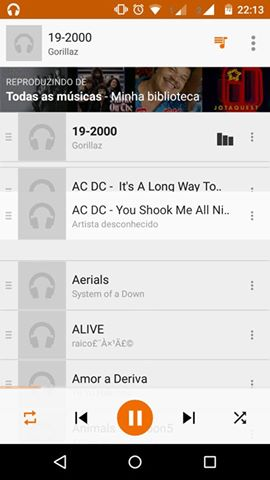
\includegraphics[width=3cm]{figuras/arrast/arrast1}
    \end{figure}
\end{block}
\end{frame}
%%%%%%%%%%%%%%%%

\begin{frame}{Padrões de Affordance}
\begin{block}{Arrastar}
    \begin{figure}
    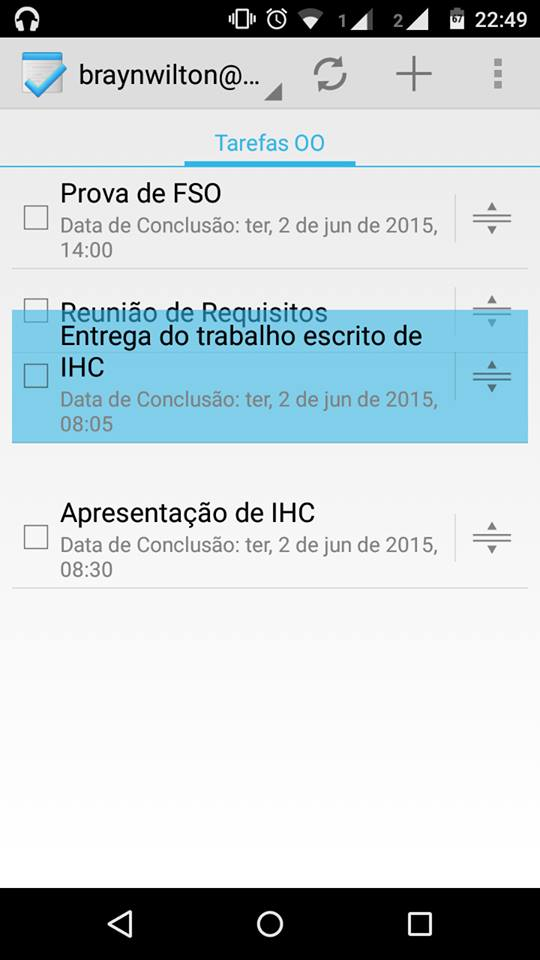
\includegraphics[width=3cm]{figuras/arrast/arrast3}
    \end{figure}
\end{block}
\end{frame}
%%%%%%%%%%%%%%%%

\begin{frame}{Padrões de Affordance}
\begin{block}{Arrastar}
    \begin{figure}
    
\includegraphics[width=3cm]{figuras/arrast/arrast2}
    \end{figure}
\end{block}
\end{frame}
%%%%%%%%%%%%%%%%